\documentclass[report]{jlreq}
\usepackage{../../global}
\usepackage{./local}
\subfiletrue
\def\assetspath{../}
%\makeindex
\begin{document}

\chapter{力学系}

\section{定義と基本的性質}

\begin{definition}[5.1.1 力学系]
    $t$を陽に含まない連立1階常微分方程式
    \begin{equation}
        \bm{y}' = \bm{f}(\bm{y})
    \end{equation}
    を\textbf{力学系}という。
    初期条件$\bm{y}(0) = \bm{y}_0$をみたす解を$\bm{y}(t; \bm{y}_0)$とおくとき、
    $\bm{y}(t; \bm{y}_0)$の軌跡
    \begin{equation}
        \calO(\bm{y}_0) \coloneqq \{ \bm{y}(t; \bm{y}_0) \mid t \in \R \}
    \end{equation}
    を$\bm{y}_0$を通る\textbf{解軌道}という。
\end{definition}

\begin{definition}
    $\bm{f}(P) = \bm{o}$をみたす点$P$を\textbf{平衡点}という。
    このとき$\bm{y} \equiv P$は解なので、$\{P\}$は軌道である。
\end{definition}

\begin{proposition}[5.1.2]
    $\bm{y}(t; \bm{y_0})$は$(t, \bm{y}_0)$に関し連続であり、
    \begin{enumerate}
        \item $\bm{y}(0; \bm{y}_0) = \bm{y}_0$
        \item $\bm{y}(t; \bm{y}(s; \bm{y}_0)) = \bm{y}(t + s; \bm{y}_0)$
    \end{enumerate}
\end{proposition}

\begin{proof}
    連続性は系1.2.9で示した。
    (1)は定義5.1.1から明らか。
    (2)は$t = 0$での一致と解の一意性から従う。
\end{proof}

\begin{proposition}[5.1.3]
    力学系の2つの軌道は共有点を持たないか、完全に一致するかのいずれかである。
\end{proposition}

\begin{proof}
    $\calO(\bm{y}_1)$と$\calO(\bm{y}_2)$が共有点$\bm{y}_0$を持つとすれば、
    $\calO(\bm{y}_0)$はいずれの解軌道とも一致する。
\end{proof}


\section{平衡点の安定性}

\begin{definition}[5.2.1]
    力学系の平衡点$P$に対し
    \begin{enumerate}
        \item $P$が\textbf{安定}であるとは、$\forall \eps > 0$に対し$\exists \delta > 0$\quad s.t.
            \begin{equation}
                \| \bm{y}_0 - P \| < \delta
                \quad \Longrightarrow \quad
                \| \bm{y}(t; \bm{y}_0) - P \| < \eps \quad (\forall t \ge 0)
            \end{equation}
            が成り立つことである。
            すなわち、初期位置を充分近くとれば$P$の$\eps$-近傍に含まれる
            軌道が存在するということである。
        \item $P$が\textbf{不安定}であるとは、安定でないことである。
        \item $P$が\textbf{漸近安定}であるとは、安定であって、$\exists \delta_0 > 0$\quad s.t.
            \begin{equation}
                \| \bm{y}_0 - P \| < \delta_0
                \quad \Longrightarrow \quad
                \| \bm{y}(t; \bm{y}_0) - P \| \to 0 \quad (t \to \infty)
            \end{equation}
            が成り立つことである。
            すなわち、初期位置を充分近くとれば軌道は
            どんどん$P$に近づいていくということである。
    \end{enumerate}
\end{definition}

平衡点$P$が安定であることは$P$への収束を要求しないため、漸近安定よりも弱い概念である。

\begin{definition}[線型化方程式]
    力学系$\bm{y}' = \bm{f}(\bm{y})$に対し
    $\bm{v} \coloneqq \bm{y} - P$とおくとき、平衡点$P$の周りでの方程式
    \begin{equation}
        \bm{v}' = A \bm{v},\quad
        A \coloneq\bm{f}'(P) 
        \label{5:eq:1}
    \end{equation}
    を$P$における\textbf{線型化方程式}といい、$A$を\textbf{線型化行列}という。
\end{definition}

定義から明らかに、線型化方程式は定数係数連立1階線型微分方程式である。
$\bm{f}(P) = 0$に注意すれば、式(\ref{5:eq:1})の右辺は$P$の周りでの$\bm{v}$の1次近似になっている。

\begin{proposition}[5.2.2]
    力学系$\bm{y}' = \bm{f}(\bm{y})\,\cdots\text{(1)}$の
    平衡点$P$における線型化方程式を$\bm{v}' = A \bm{v} \; \cdots \text{(2)}$とし、
    線型化行列$A$の固有値を$\lambda_1, \dots, \lambda_n$とする。
    このとき
    \begin{enumerate}
        \item $\forall i$に対し$\Re \lambda_i < 0$ならば
            (2) は$\bm{o}$において漸近安定
        \item $\exists i$に対し$\Re \lambda_i > 0$ならば
            (2) は$\bm{o}$において不安定
    \end{enumerate}
\end{proposition}

この命題は、固有値に$0$が含まれていない限りでは、
(1) の平衡点$P$における安定性と解釈できることが知られている。

\begin{proof}
    定数係数連立1階線型微分方程式の性質により、
    初期値$\bm{v}_0$に対応する解は$e^{xA} \bm{v}_0$である。
    ここで行列$e^{xJ} = Q^{-1} e^{xA} Q$は
    $J$のジョルダン細胞に対応するブロック対角成分を持つが、
    各ブロックのノルムは、そのブロックに対応する固有値が正か負かに応じて
    $t \to \infty$で$\infty$か$0$に至る。
    この性質を用いて命題の主張が示される。
\end{proof}





\section{2次元力学系の平衡点}

2次元力学系$\bm{y}' = \bm{f}(\bm{y})$について、
平衡点の周りでの解のふるまいを考えよう。
簡単のため、線型化方程式$\bm{v}' = A \bm{v}$の線型化行列$A$の
固有値$\lambda_1, \lambda_2$は相異なるものとする。
$\lambda_1, \lambda_2$に対応する固有ベクトルをそれぞれ$\bm{p}_1, \bm{p}_2$とおくと、
\begin{equation}
    \bm{v}(t) = \alpha_1(t) \bm{p}_1 + \alpha_2(t) \bm{p}_2
\end{equation}
と表すことができ、したがって、$\lambda_1, \lambda_2$が$A$の固有値であることから
\begin{equation}
    \bm{v}' = A \bm{v}
        = \lambda_1 \alpha_1(t) \bm{p}_1
        + \lambda_2 \alpha_2(t) \bm{p}_2
\end{equation}
すなわち
\begin{equation}
    \alpha_i'(t) = \lambda_i \alpha_i(t)
\end{equation}
である。
これを解くと
\begin{equation}
    \alpha_i(t) = C_i e^{\lambda_i t}
\end{equation}
なので
\begin{equation}
    \bm{v}
        = C_1 e^{\lambda_1 t} \bm{p}_1
        + C_2 e^{\lambda_2 t} \bm{p}_2
\end{equation}
と書くことができ、この表式を利用して解のふるまいを考えることができる。

\subsection{$\lambda_1, \lambda_2 > 0$のとき}

$e^{\lambda_i t} \to \infty\, (t \to \infty)$なので、
解のふるまいは図(\ref{5:fig:1})のようになる。
このような平衡点$P$を\textbf{不安定結節点}という。

\begin{figure}[H]
    \centering
    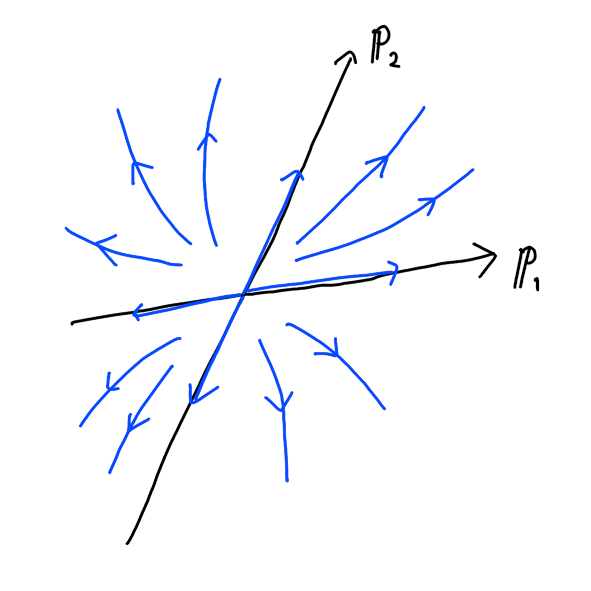
\includegraphics[height=5cm]{\assetspath assets/v1.png}
    \caption{不安定結節点}
    \label{5:fig:1}
\end{figure}

\subsection{$\lambda_1 > 0 > \lambda_2$のとき}

$e^{\lambda_1 t} \to \infty,\, e^{\lambda_2 t} \to 0\, (t \to \infty)$なので、
解のふるまいは図(\ref{5:fig:2})のようになる。
このような平衡点$P$を\textbf{鞍点}という。

\begin{figure}[H]
    \centering
    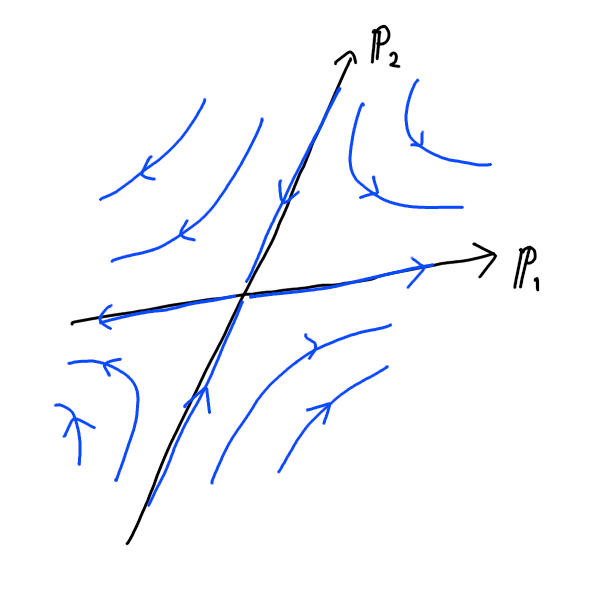
\includegraphics[width=5cm]{\assetspath assets/v2.png}
    \caption{鞍点}
    \label{5:fig:2}
\end{figure}

\subsection{$\lambda_1, \lambda_2 < 0$のとき}

$e^{\lambda_i t} \to 0\, (t \to \infty)$なので、
解のふるまいは図(\ref{5:fig:3})のようになる。
このような平衡点$P$を\textbf{安定結節点}という。

\begin{figure}[H]
    \centering
    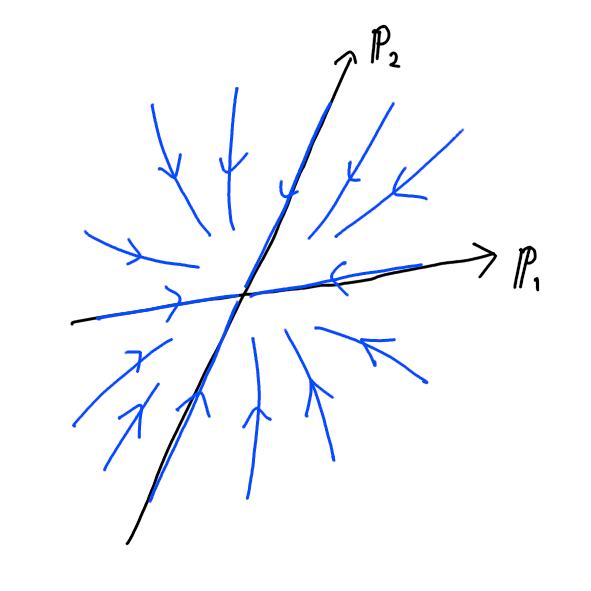
\includegraphics[width=5cm]{\assetspath assets/v3.png}
    \caption{安定結節点}
    \label{5:fig:3}
\end{figure}

\subsection{
    \texorpdfstring{%
        $\lambda_1 = \overline{\lambda_2} \not\in \R,\, \Re \lambda_i > 0$のとき%
    }{%
        %
    }%
}

解のふるまいは図(\ref{5:fig:4})のようになる。
このような平衡点$P$を\textbf{不安定渦状点}という。

\begin{figure}[H]
    \centering
    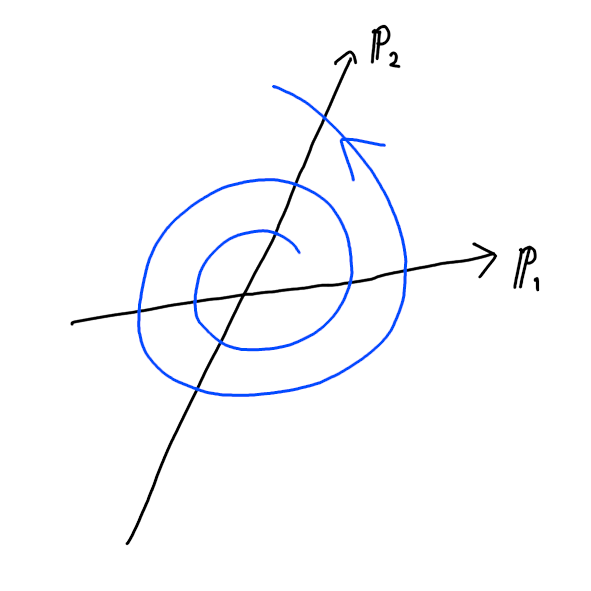
\includegraphics[width=5cm]{\assetspath assets/v4.png}
    \caption{不安定渦状点}
    \label{5:fig:4}
\end{figure}

\subsection{
    \texorpdfstring{%
        $\lambda_1 = \overline{\lambda_2} \not\in \R,\, \Re \lambda_i < 0$のとき%
    }{%
        %
    }%
}

解のふるまいは図(\ref{5:fig:5})のようになる。
このような平衡点$P$を\textbf{安定渦状点}という。

\begin{figure}[H]
    \centering
    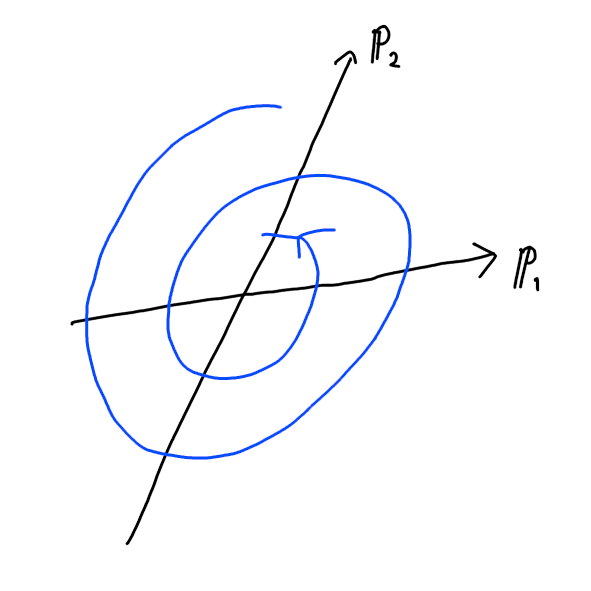
\includegraphics[width=5cm]{\assetspath assets/v5.png}
    \caption{安定渦状点}
    \label{5:fig:5}
\end{figure}

\subsection{$\Re\lambda_i = 0$の固有値があるとき}

線型化方程式の解のふるまいを用いて元の力学系の解のふるまいを判定することはできない。


\begin{problem}
    力学系
    \begin{equation}
        \begin{cases}
            x' = (1 - y) x \\
            y' = (1 + 2x) y
        \end{cases}
    \end{equation}
    の解で$x(0), y(0) > 0$をみたすものは
    $\forall t \in \R$に対し$x(0), y(0) > 0$をみたすことを示せ。
\end{problem}

\begin{problem}
    2次元力学系
    \begin{equation}
        \begin{cases}
            x' &= (1 - x - 3y) x \\
            y' &= (1 - 3x - y) y
        \end{cases}
    \end{equation}
    の平衡点の種類を判定せよ。

    解答:不安定結節点$(0, 0)$、鞍点$(1/4, 1/4)$、安定結節点$(1, 0), (0, 1)$
\end{problem}

\begin{problem}
    教科書の問5.3, 問5.4, 問5.5を読者の演習問題とする。
\end{problem}


\end{document}